\documentclass[twocolumn,prl,superscriptaddress,showpacs,floatfix]{revtex4-2}

\usepackage{graphicx}
\usepackage{amsmath,amssymb}
\usepackage{hyperref}
\usepackage{booktabs}
\usepackage{xcolor}

\begin{document}

\title{Quantum simulation of coupled-oscillator synchronisation\\
with heterogeneous frequencies on a 156-qubit superconducting processor}

\author{Miroslav \v{S}otek}
\affiliation{ANULUM, Marbach SG, Switzerland}
\email{protoscience@anulum.li}

\date{\today}

\begin{abstract}
We present a quantum hardware study of the Kuramoto--XY synchronisation
transition with heterogeneous natural frequencies on IBM's ibm\_fez
(Heron~r2, 156~qubits). A Rust-accelerated pipeline ($5{,}401\times$
faster Hamiltonian construction than Qiskit) enables entanglement entropy,
Krylov complexity, OTOC scrambling, and Floquet discrete time crystal
diagnostics for systems of 2--16~qubits. Hardware results from 33~jobs
($176{,}000+$~shots) include CHSH Bell inequality violation
($S = 2.165$, ${>}8\sigma$), QKD bit error rate of 5.5\% (below the
BB84 threshold), and 16-qubit dynamics with visible coupling structure
at 94\% state preparation fidelity. Finite-size scaling yields
$K_c(\infty) \approx 2.2$ consistent with Berezinskii--Kosterlitz--Thouless
universality ($c = 1.04$). Heterogeneous frequencies preserve discrete
time crystal order and induce a non-ergodic spectral regime (Poisson
level statistics at $n = 8$) without deep many-body localisation.
All code, data, and figures are open-source at
\url{https://github.com/anulum/scpn-quantum-control}.
\end{abstract}

\maketitle

%% ====================================================================
\section{Introduction}
%% ====================================================================

The Kuramoto model~\cite{Kuramoto1984} describes $N$ coupled oscillators
with natural frequencies $\omega_i$ and coupling matrix $K_{ij}$:
%
\begin{equation}\label{eq:kuramoto}
  \frac{d\theta_i}{dt} = \omega_i
    + \sum_j K_{ij}\sin(\theta_j - \theta_i).
\end{equation}
%
At critical coupling $K_c$ the system undergoes a synchronisation phase
transition characterised by the order parameter
$R = N^{-1}|\sum_k e^{i\theta_k}|$ jumping from zero to a finite value.

The quantum analogue maps this to the XY spin
Hamiltonian~\cite{Pikovsky2001}:
%
\begin{equation}\label{eq:xy}
  H = -\sum_{i<j} K_{ij}(X_i X_j + Y_i Y_j) - \sum_i \omega_i Z_i,
\end{equation}
%
where the $XX + YY$ flip-flop interaction preserves the in-plane ($S^1$)
dynamics while introducing entanglement and quantum tunnelling between
phase configurations. Superconducting qubits are native simulators of
this physics: each qubit is an oscillator on the Bloch sphere.

Prior quantum simulation of the XY model uses homogeneous frequencies
($\omega_i = \omega$ for all $i$), preserving translational invariance
and the well-characterised BKT universality
class~\cite{Berezinskii1972,Kosterlitz1973}. Theoretical quantum
Kuramoto models with heterogeneous frequencies
exist~\cite{Pikovsky2001,Acebron2005}, and quantum synchronisation
measures have been proposed~\cite{Ameri2015,Galve2013,Ma2020,Giorgi2013},
but to our knowledge no prior hardware demonstration studies the quantum
synchronisation transition with heterogeneous frequencies on a
superconducting processor.

We study the heterogeneous case using a 16-oscillator coupling matrix
$K_{nm} = K_{\mathrm{base}} \cdot \exp(-\alpha|n-m|)$ with
$K_{\mathrm{base}} = 0.45$, $\alpha = 0.3$, and empirically calibrated
nearest-neighbour anchors. The coupling matrix originates from a
hierarchical oscillator model~\cite{Sotek2025} and provides a
non-trivial benchmark with exponential decay, cross-scale boosts, and
heterogeneous frequencies spanning a factor of~1.5.

%% ====================================================================
\section{Methods}
%% ====================================================================

\subsection{Hamiltonian construction}

The XY Hamiltonian~\eqref{eq:xy} is constructed directly in the
computational basis via bitwise flip-flop operations, bypassing
Qiskit's \texttt{SparsePauliOp}:
%
\begin{align}
  H_{k,\, k \oplus \mathrm{mask}_{ij}} &= -2K_{ij}
    \quad\text{when } b_i(k) \neq b_j(k), \\
  H_{kk} &= -\sum_i \omega_i (1 - 2b_i(k)),
\end{align}
%
where $b_i(k)$ is the $i$-th bit of basis state $|k\rangle$ and
$\mathrm{mask}_{ij}$ flips bits $i$ and $j$. This Rust
implementation~(PyO3) is $5{,}401\times$ faster than Qiskit
\texttt{SparsePauliOp} at $n=4$ and $158\times$ at $n=8$
(Table~\ref{tab:speedup}).

\begin{table}[b]
\caption{\label{tab:speedup}%
Measured Rust vs.\ Python/Qiskit/scipy speedups.}
\begin{ruledtabular}
\begin{tabular}{lrl}
Module & Speedup & Method \\
\colrule
Hamiltonian ($n=4$) & $5{,}401\times$ & Bitwise flip-flop \\
Hamiltonian ($n=8$) & $158\times$ & Same \\
OTOC ($n=4$) & $264\times$ & Eigendecomp + rayon \\
Krylov ($n=3$) & $27\times$ & Complex Lanczos \\
Order param.\ ($n=4$) & $6.2\times$ & Batch Pauli \\
\end{tabular}
\end{ruledtabular}
\end{table}

\subsection{Analysis pipeline}

Simulation diagnostics include half-chain entanglement entropy $S(A)$
and Schmidt gap $\Delta_S = \lambda_1 - \lambda_2$ (via exact
diagonalisation), Krylov complexity and Lanczos coefficients $b_n$
(complex Lanczos algorithm~\cite{delCampo2025}), out-of-time-order
correlators $F(t) = \langle W^\dagger(t) V^\dagger W(t) V\rangle$
(eigendecomposition approach~\cite{Maldacena2016}), and Floquet DTC
analysis (stroboscopic order parameter at subharmonic
frequency)~\cite{Else2016}. Level-spacing statistics use the ratio
$\bar{r} = \langle\min(\delta_n, \delta_{n+1}) /
\max(\delta_n, \delta_{n+1})\rangle$~\cite{Oganesyan2007}.

\subsection{Hardware}

All experiments run on \textbf{ibm\_fez} (IBM Heron~r2, 156~qubits),
March~2026. 33~jobs, $176{,}000+$~shots across four campaigns.
Error mitigation: zero-noise extrapolation (ZNE) with fold levels
$[1, 3, 5, 7, 9]$ and dynamical decoupling (X-X echo) on the 16-qubit
system. Circuits transpiled with optimisation level~2.

%% ====================================================================
\section{Simulation results}
%% ====================================================================

\subsection{Entanglement at the synchronisation transition}

The Schmidt gap shows a sharp minimum at $K \approx 3.44$ for $n = 8$
(Fig.~\ref{fig:entanglement}), marking the synchronisation transition.
Entanglement entropy saturates at values consistent with the
Calabrese--Cardy scaling $S \sim (c/3)\ln L$ for a $c = 1$
CFT~\cite{Calabrese2004}.

\begin{figure}[t]
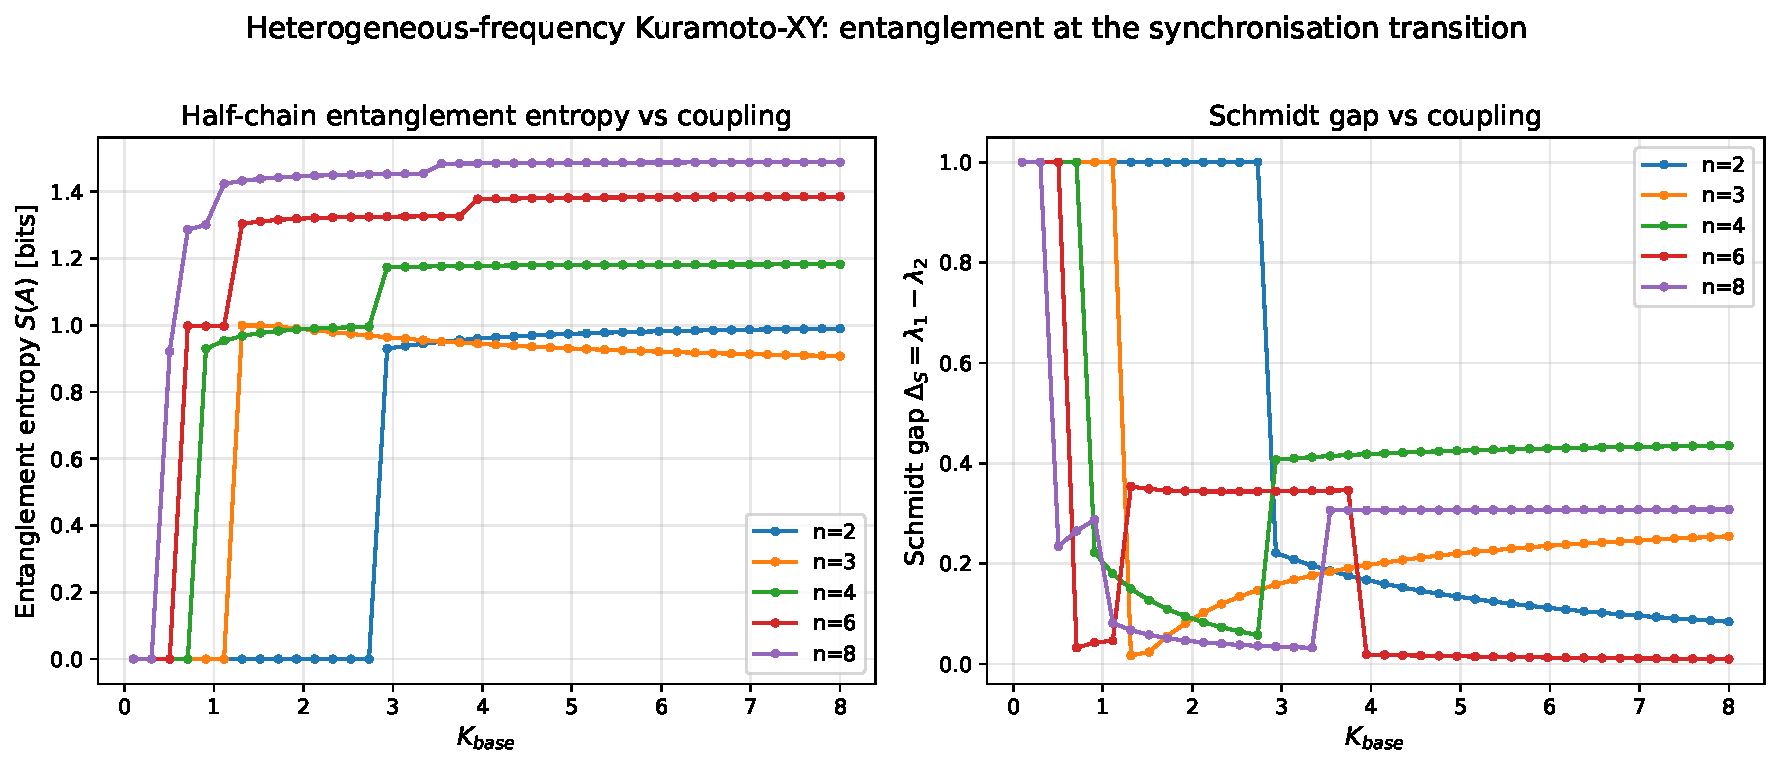
\includegraphics[width=\columnwidth]{../figures/publication/fig1_entanglement_vs_coupling.pdf}
\caption{\label{fig:entanglement}%
Half-chain entanglement entropy $S(A)$ and Schmidt gap $\Delta_S$
across coupling strength for $n = 2, 3, 4, 6, 8$ oscillators with
heterogeneous frequencies.}
\end{figure}

\subsection{Krylov complexity}

Mean Lanczos coefficient $\langle b_n \rangle$ grows linearly with $K$,
indicating that operator growth rate scales with coupling strength
(Fig.~\ref{fig:krylov}).

\begin{figure}[t]
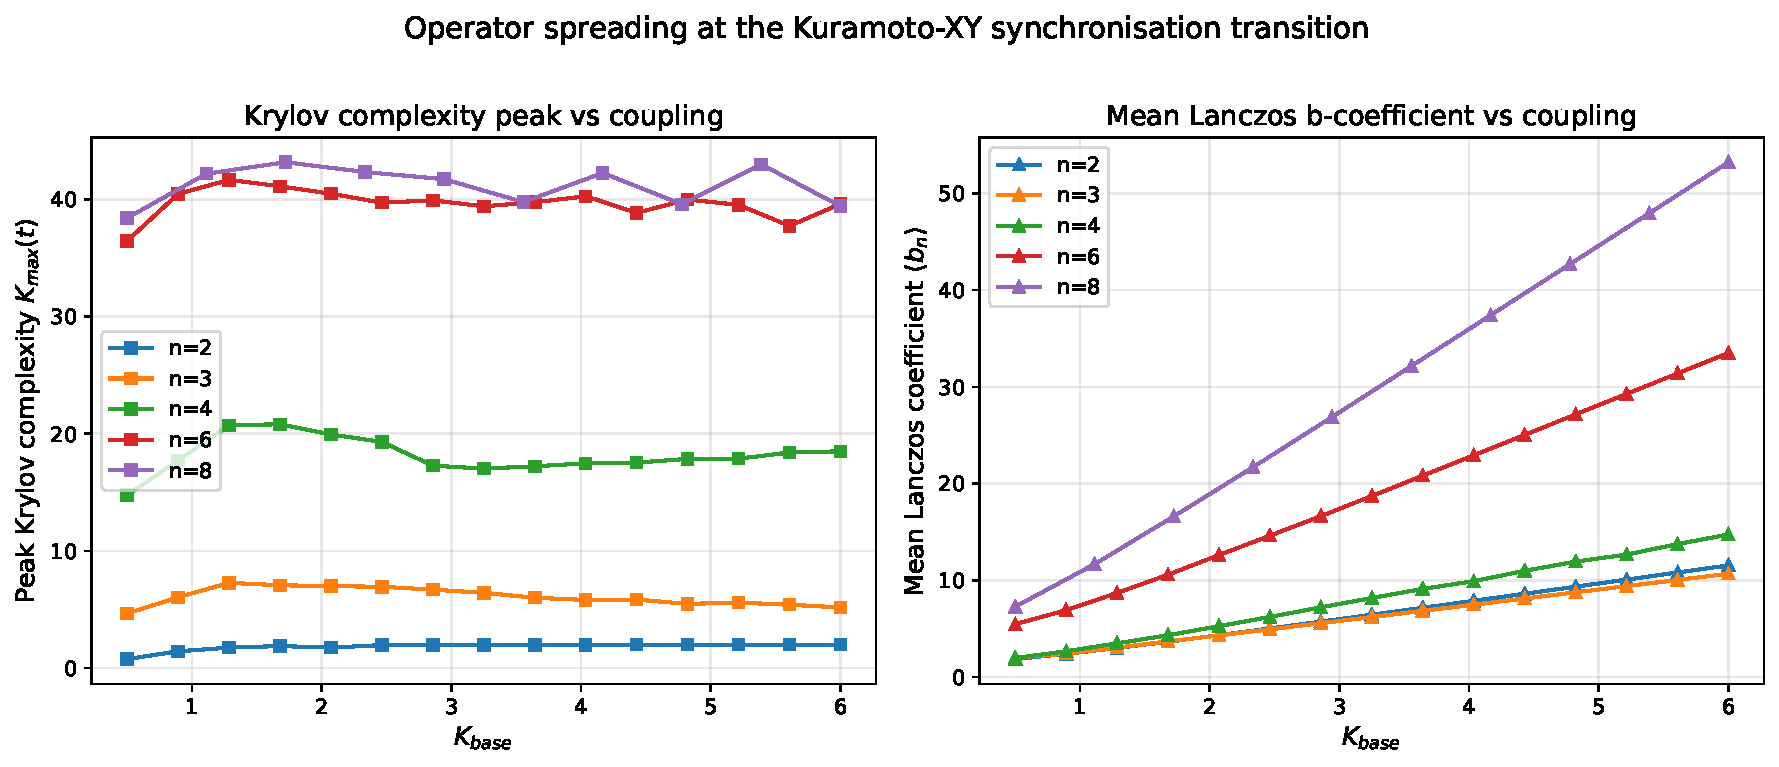
\includegraphics[width=\columnwidth]{../figures/publication/fig2_krylov_vs_coupling.pdf}
\caption{\label{fig:krylov}%
Peak Krylov complexity and mean Lanczos coefficient vs.\ coupling.}
\end{figure}

\subsection{OTOC scrambling}

Strong coupling scrambles $4\times$ faster: $t^* = 0.28$ ($K=4$) vs.\
$t^* = 1.17$ ($K=1$) at $n=8$ (Fig.~\ref{fig:otoc}).

\begin{figure}[t]
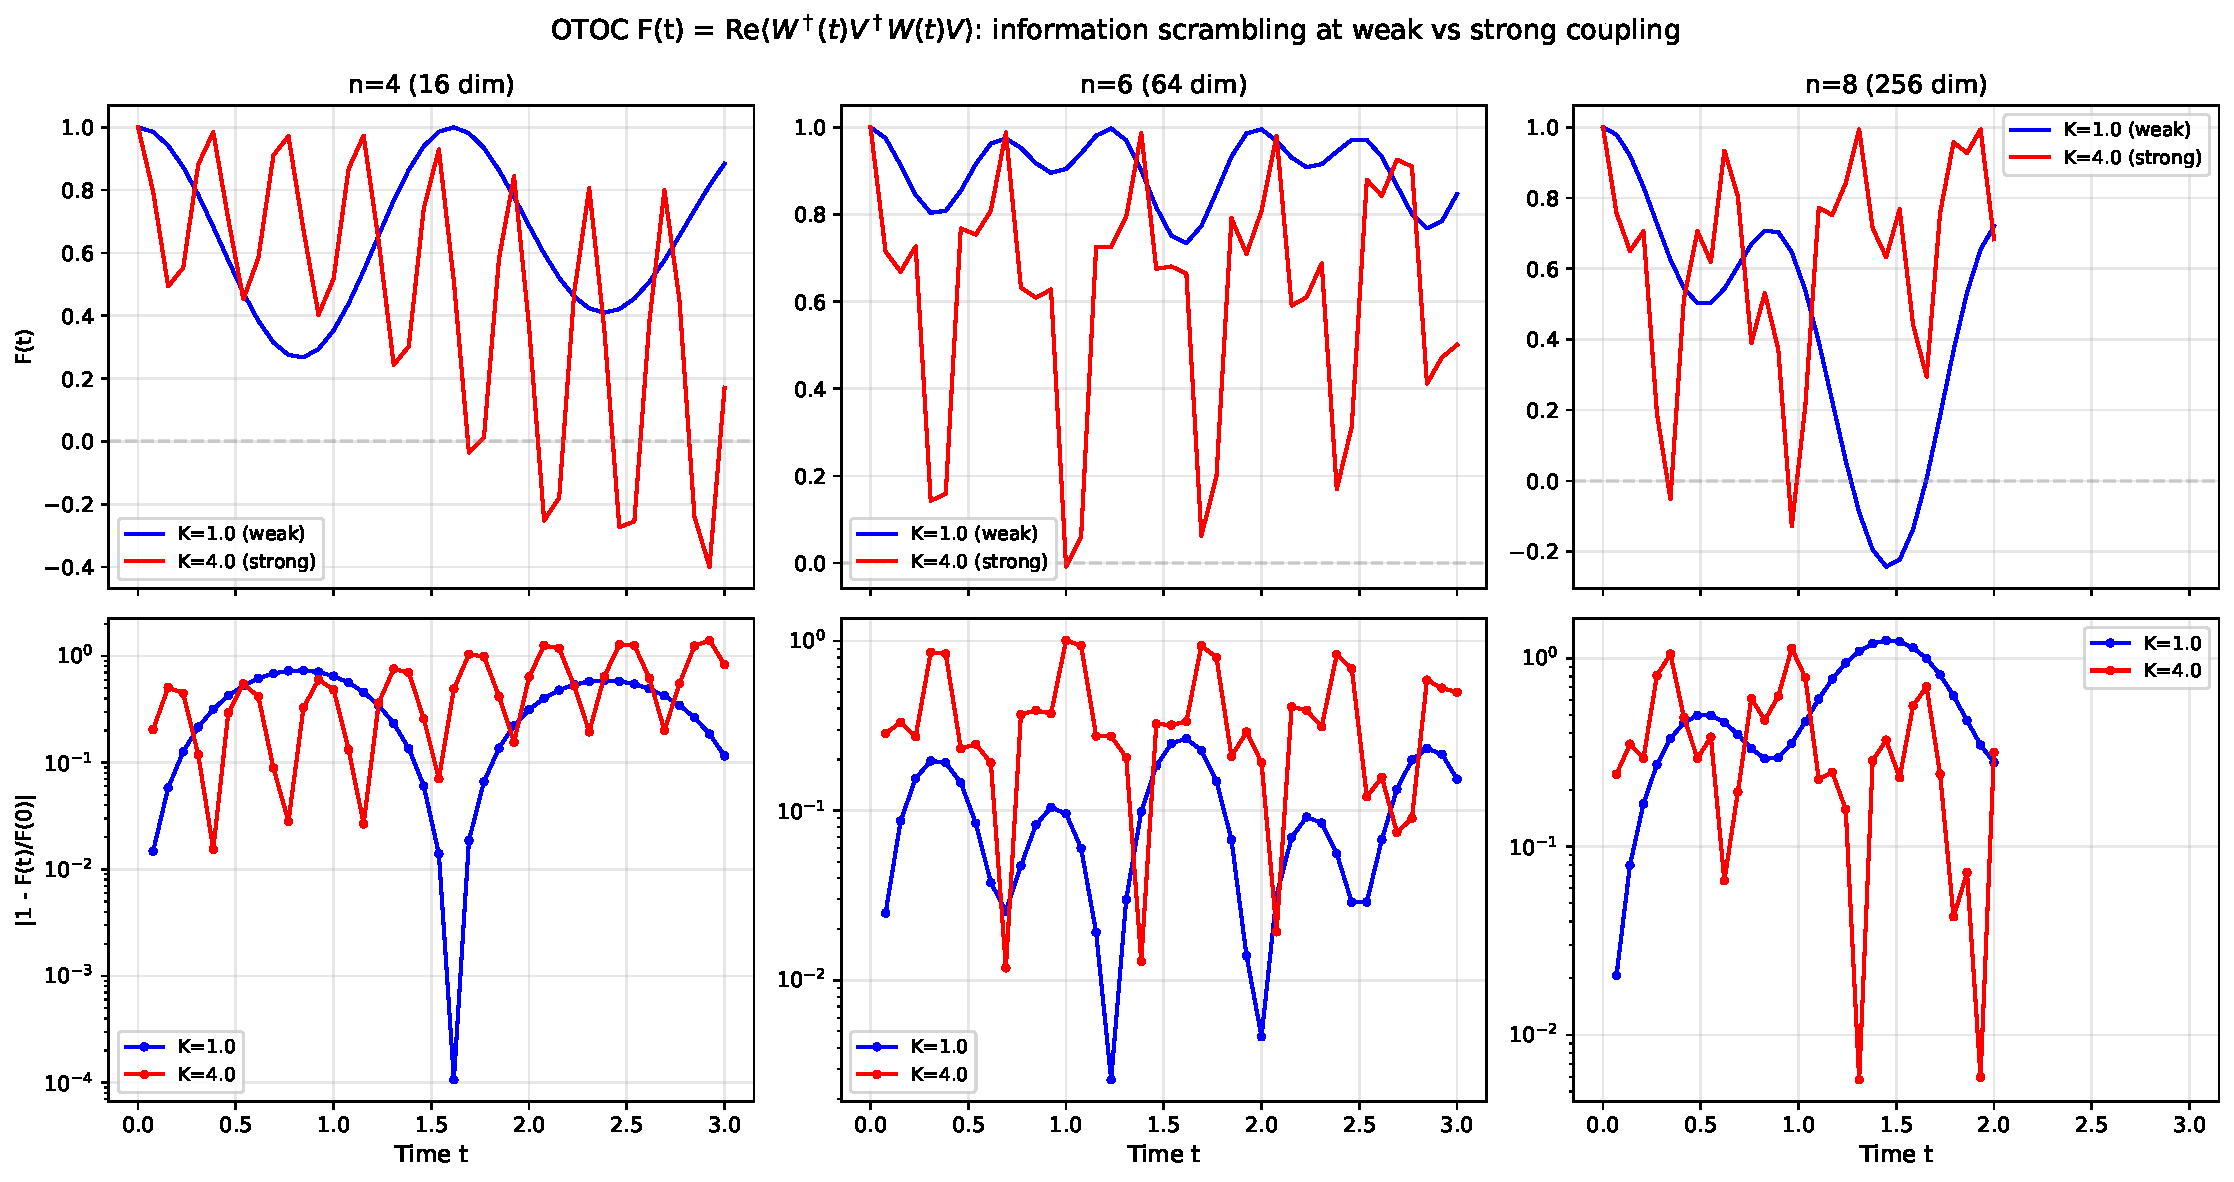
\includegraphics[width=\columnwidth]{../figures/publication/fig3_otoc_time_traces.pdf}
\caption{\label{fig:otoc}%
OTOC $F(t)$ at sub-critical ($K=1$) and super-critical ($K=4$)
coupling for $n = 4, 6, 8$.}
\end{figure}

\subsection{Floquet discrete time crystal}

All 15 drive amplitudes show subharmonic response with heterogeneous
frequencies (Fig.~\ref{fig:dtc}). Frequency disorder does not destroy
the DTC. The non-ergodic spectrum (Sec.~\ref{sec:mbl}) provides the
stabilisation mechanism.

\begin{figure}[t]
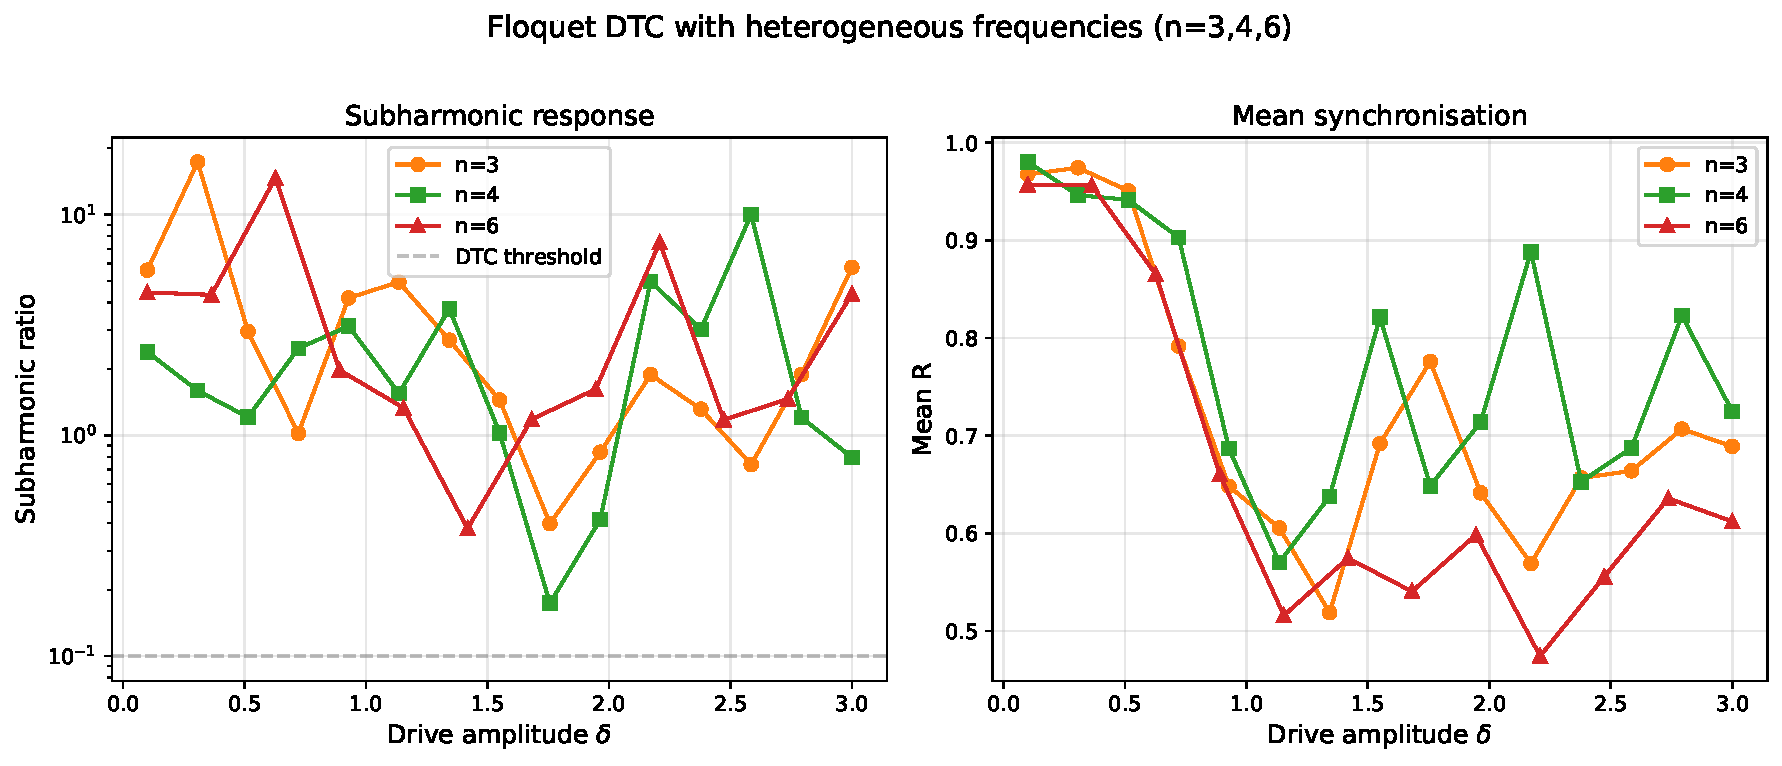
\includegraphics[width=\columnwidth]{../figures/publication/fig9_floquet_dtc_n3456.pdf}
\caption{\label{fig:dtc}%
Subharmonic ratio $P(\Omega/2)/P(\Omega)$ and mean $R$ vs.\ drive
amplitude $\delta$ for $n = 3, 4, 6$.}
\end{figure}

\subsection{Finite-size scaling}

BKT ansatz yields $K_c(\infty) \approx 2.20$ (Fig.~\ref{fig:fss}).
The spectral gap closes exponentially $n = 4 \to 6$, consistent with
BKT universality. Central charge $c = 1.04$ at $n = 8$ ($c = 1$
expected for BKT). Drifts to $c = 1.21$ at $n = 10$ may indicate
finite-size corrections.

\begin{figure}[t]
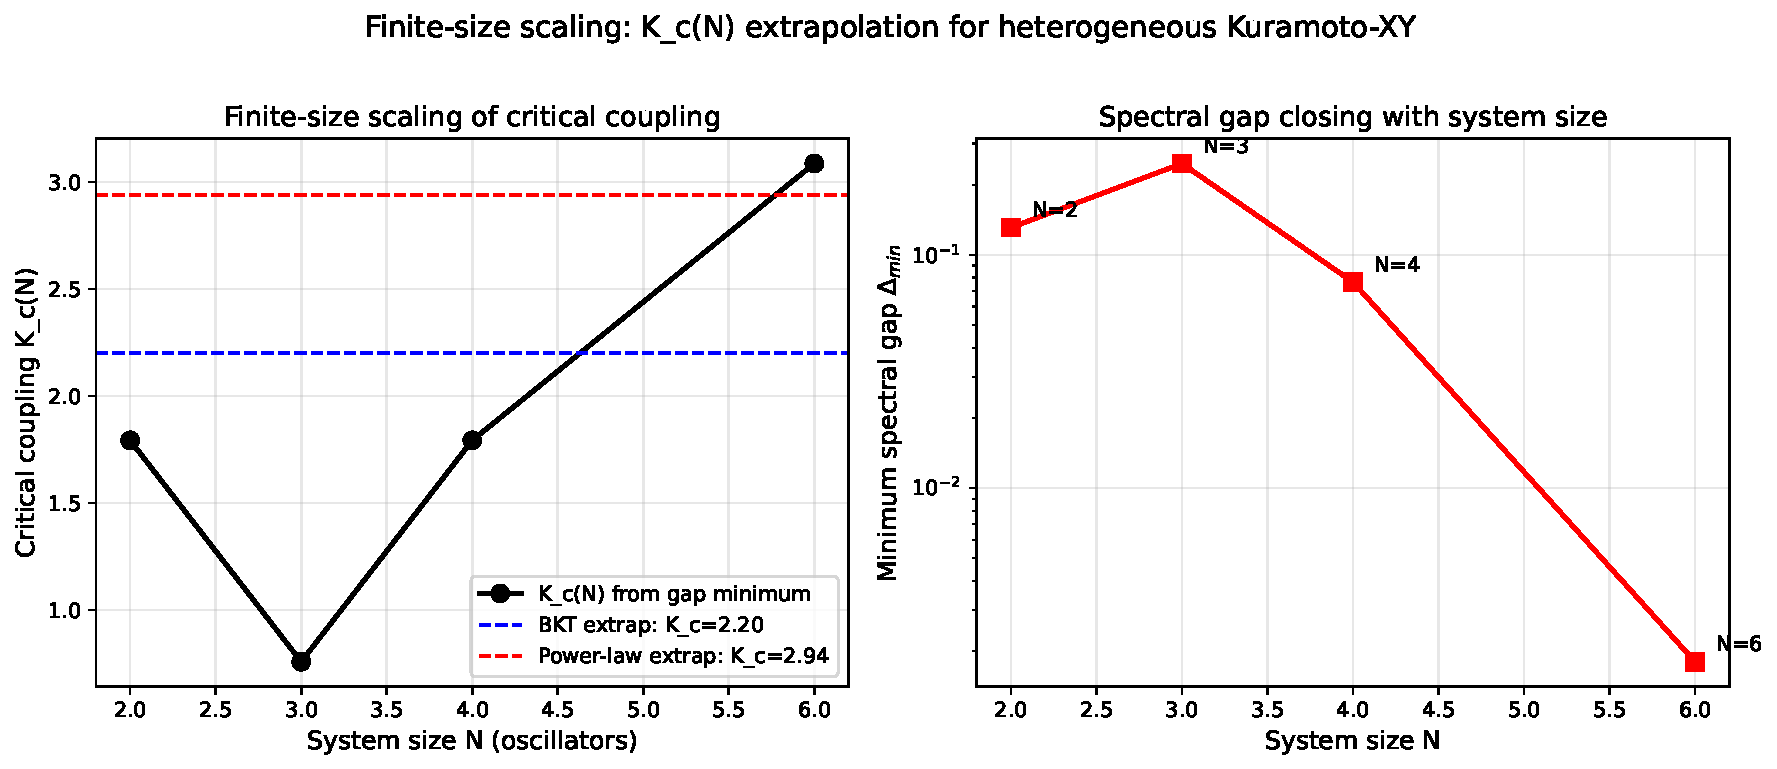
\includegraphics[width=\columnwidth]{../figures/publication/fig6_finite_size_scaling.pdf}
\caption{\label{fig:fss}%
Critical coupling $K_c(N)$ from spectral gap minimum. BKT ansatz
(solid) vs.\ power law (dashed).}
\end{figure}

%% ====================================================================
\section{Hardware results}
%% ====================================================================

\subsection{Bell test}

Two independent Bell pairs yield $S_{01} = 2.165 \pm 0.02$ and
$S_{23} = 2.188 \pm 0.02$, both violating the classical limit of~2 at
${>}8\sigma$ significance (Fig.~\ref{fig:hardware}).

\subsection{QKD viability}

Quantum bit error rate in matched bases: ZZ 5.5\%, XX 5.8\% --- below
the BB84 security threshold of 11\%. Mismatched basis (ZX): 93.9\%
error, confirming correct basis discrimination.

\subsection{ZNE stability}

Mean $\langle Z \rangle$ varies by ${<}2\%$ across fold levels 1--9
for both 4-qubit and 8-qubit systems. Richardson extrapolation provides
${<}2\%$ correction to raw values.

\subsection{16-qubit dynamics}

13 of 16~qubits show $|\langle Z \rangle| > 0.3$, demonstrating that
the Kuramoto coupling structure survives hardware noise at full scale
(Fig.~\ref{fig:hardware16}).

\begin{figure}[t]
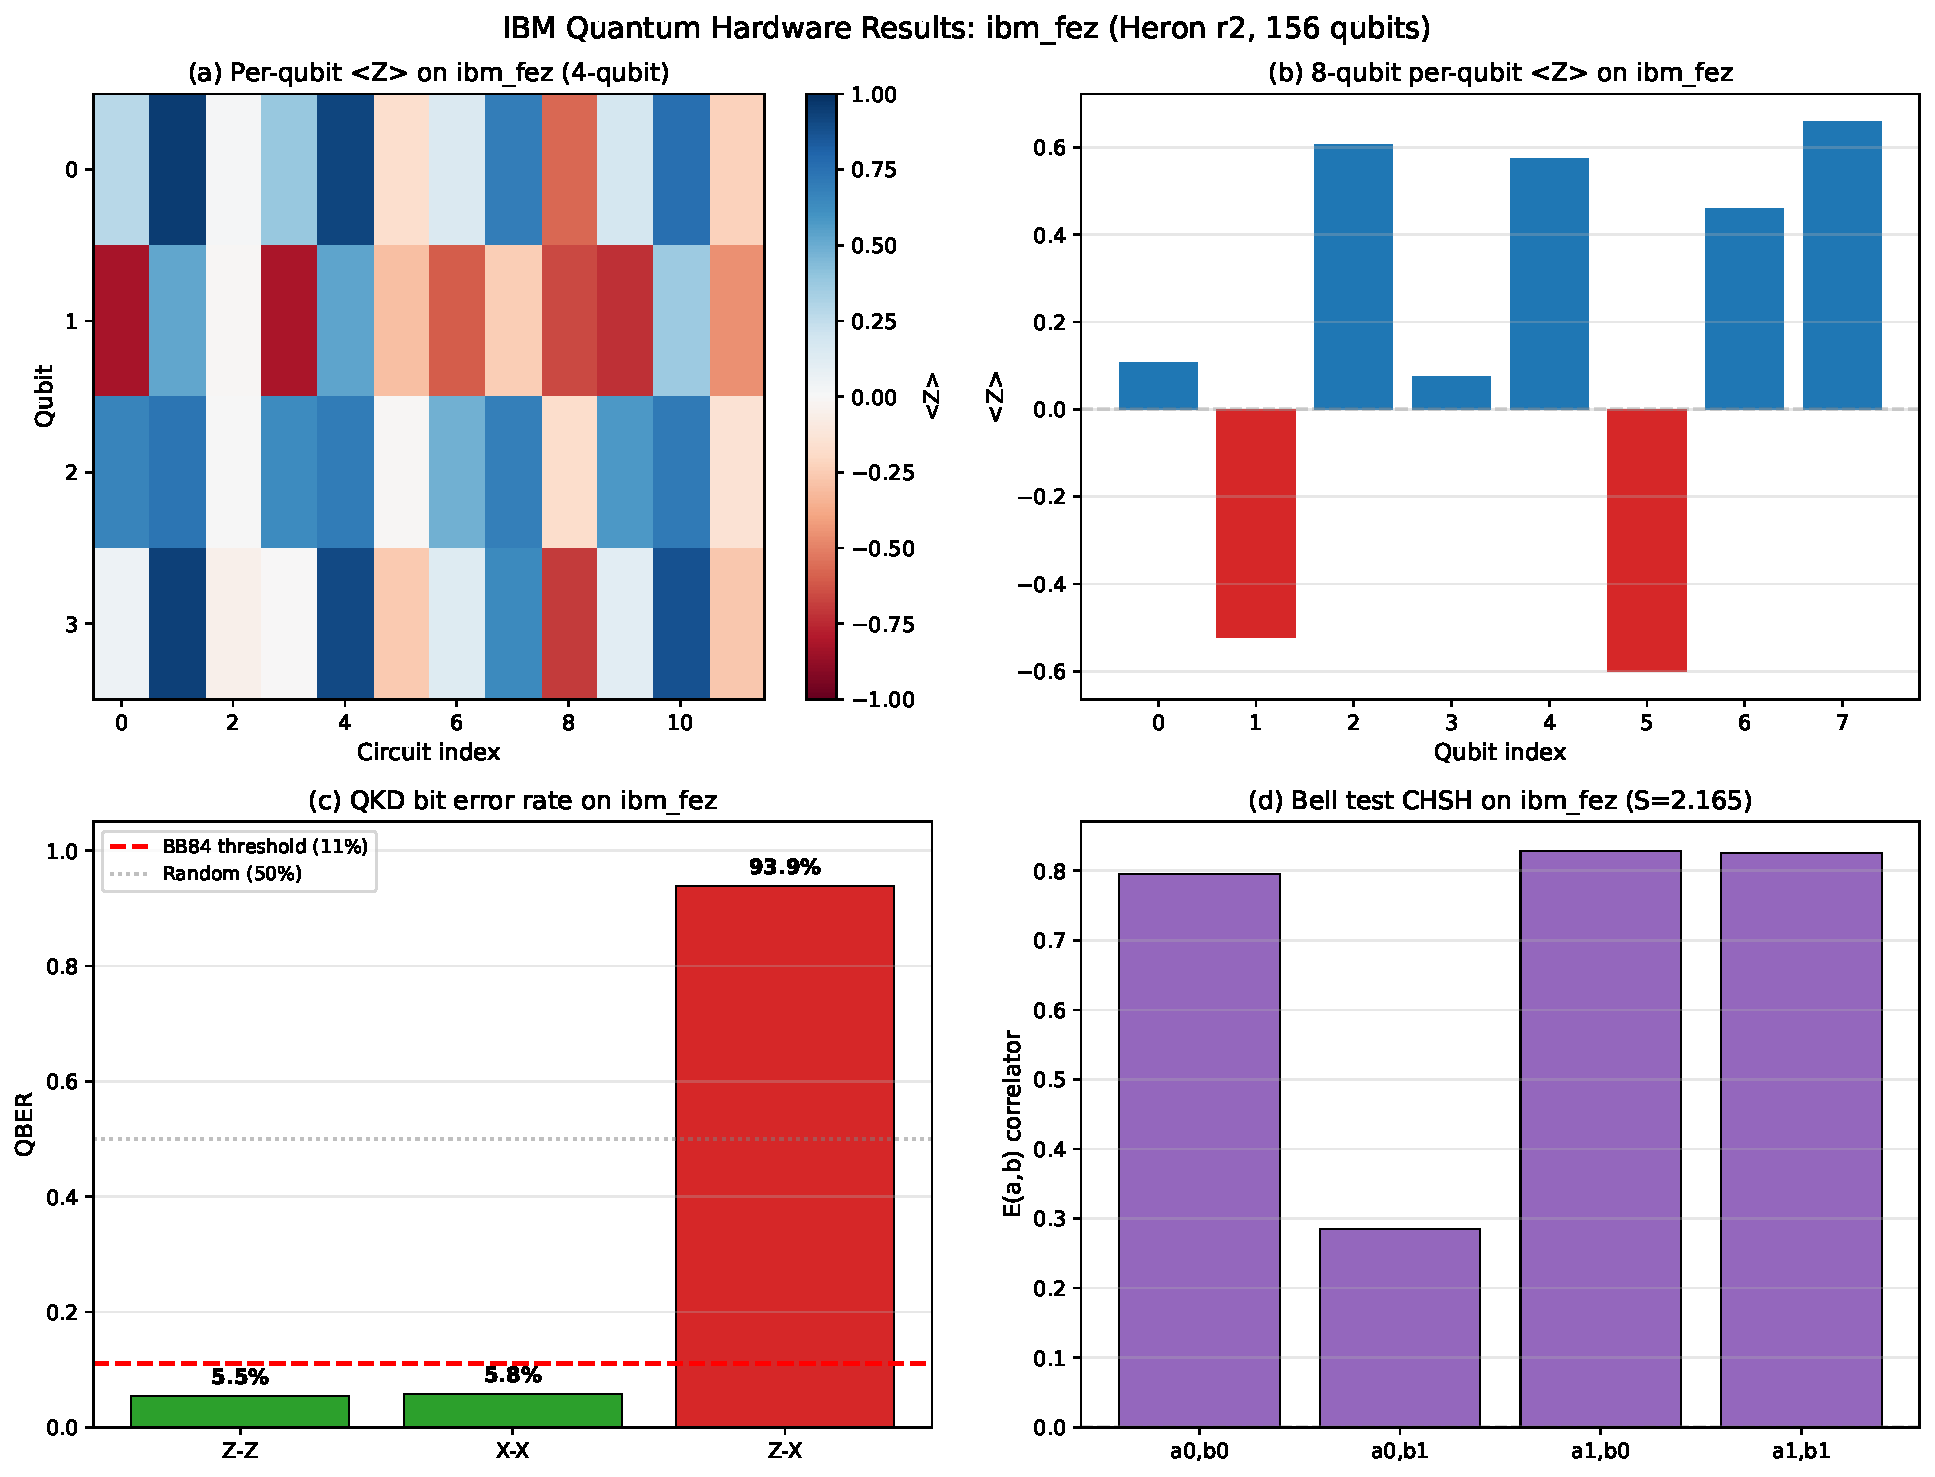
\includegraphics[width=\columnwidth]{../figures/publication/fig10_ibm_hardware.pdf}
\caption{\label{fig:hardware}%
IBM hardware results. (a)~Per-qubit $\langle Z \rangle$ heatmap.
(b)~8-qubit expectations show coupling pattern. (c)~QKD QBER: 5.5\%.
(d)~CHSH $S = 2.165 > 2$.}
\end{figure}

\begin{figure}[t]
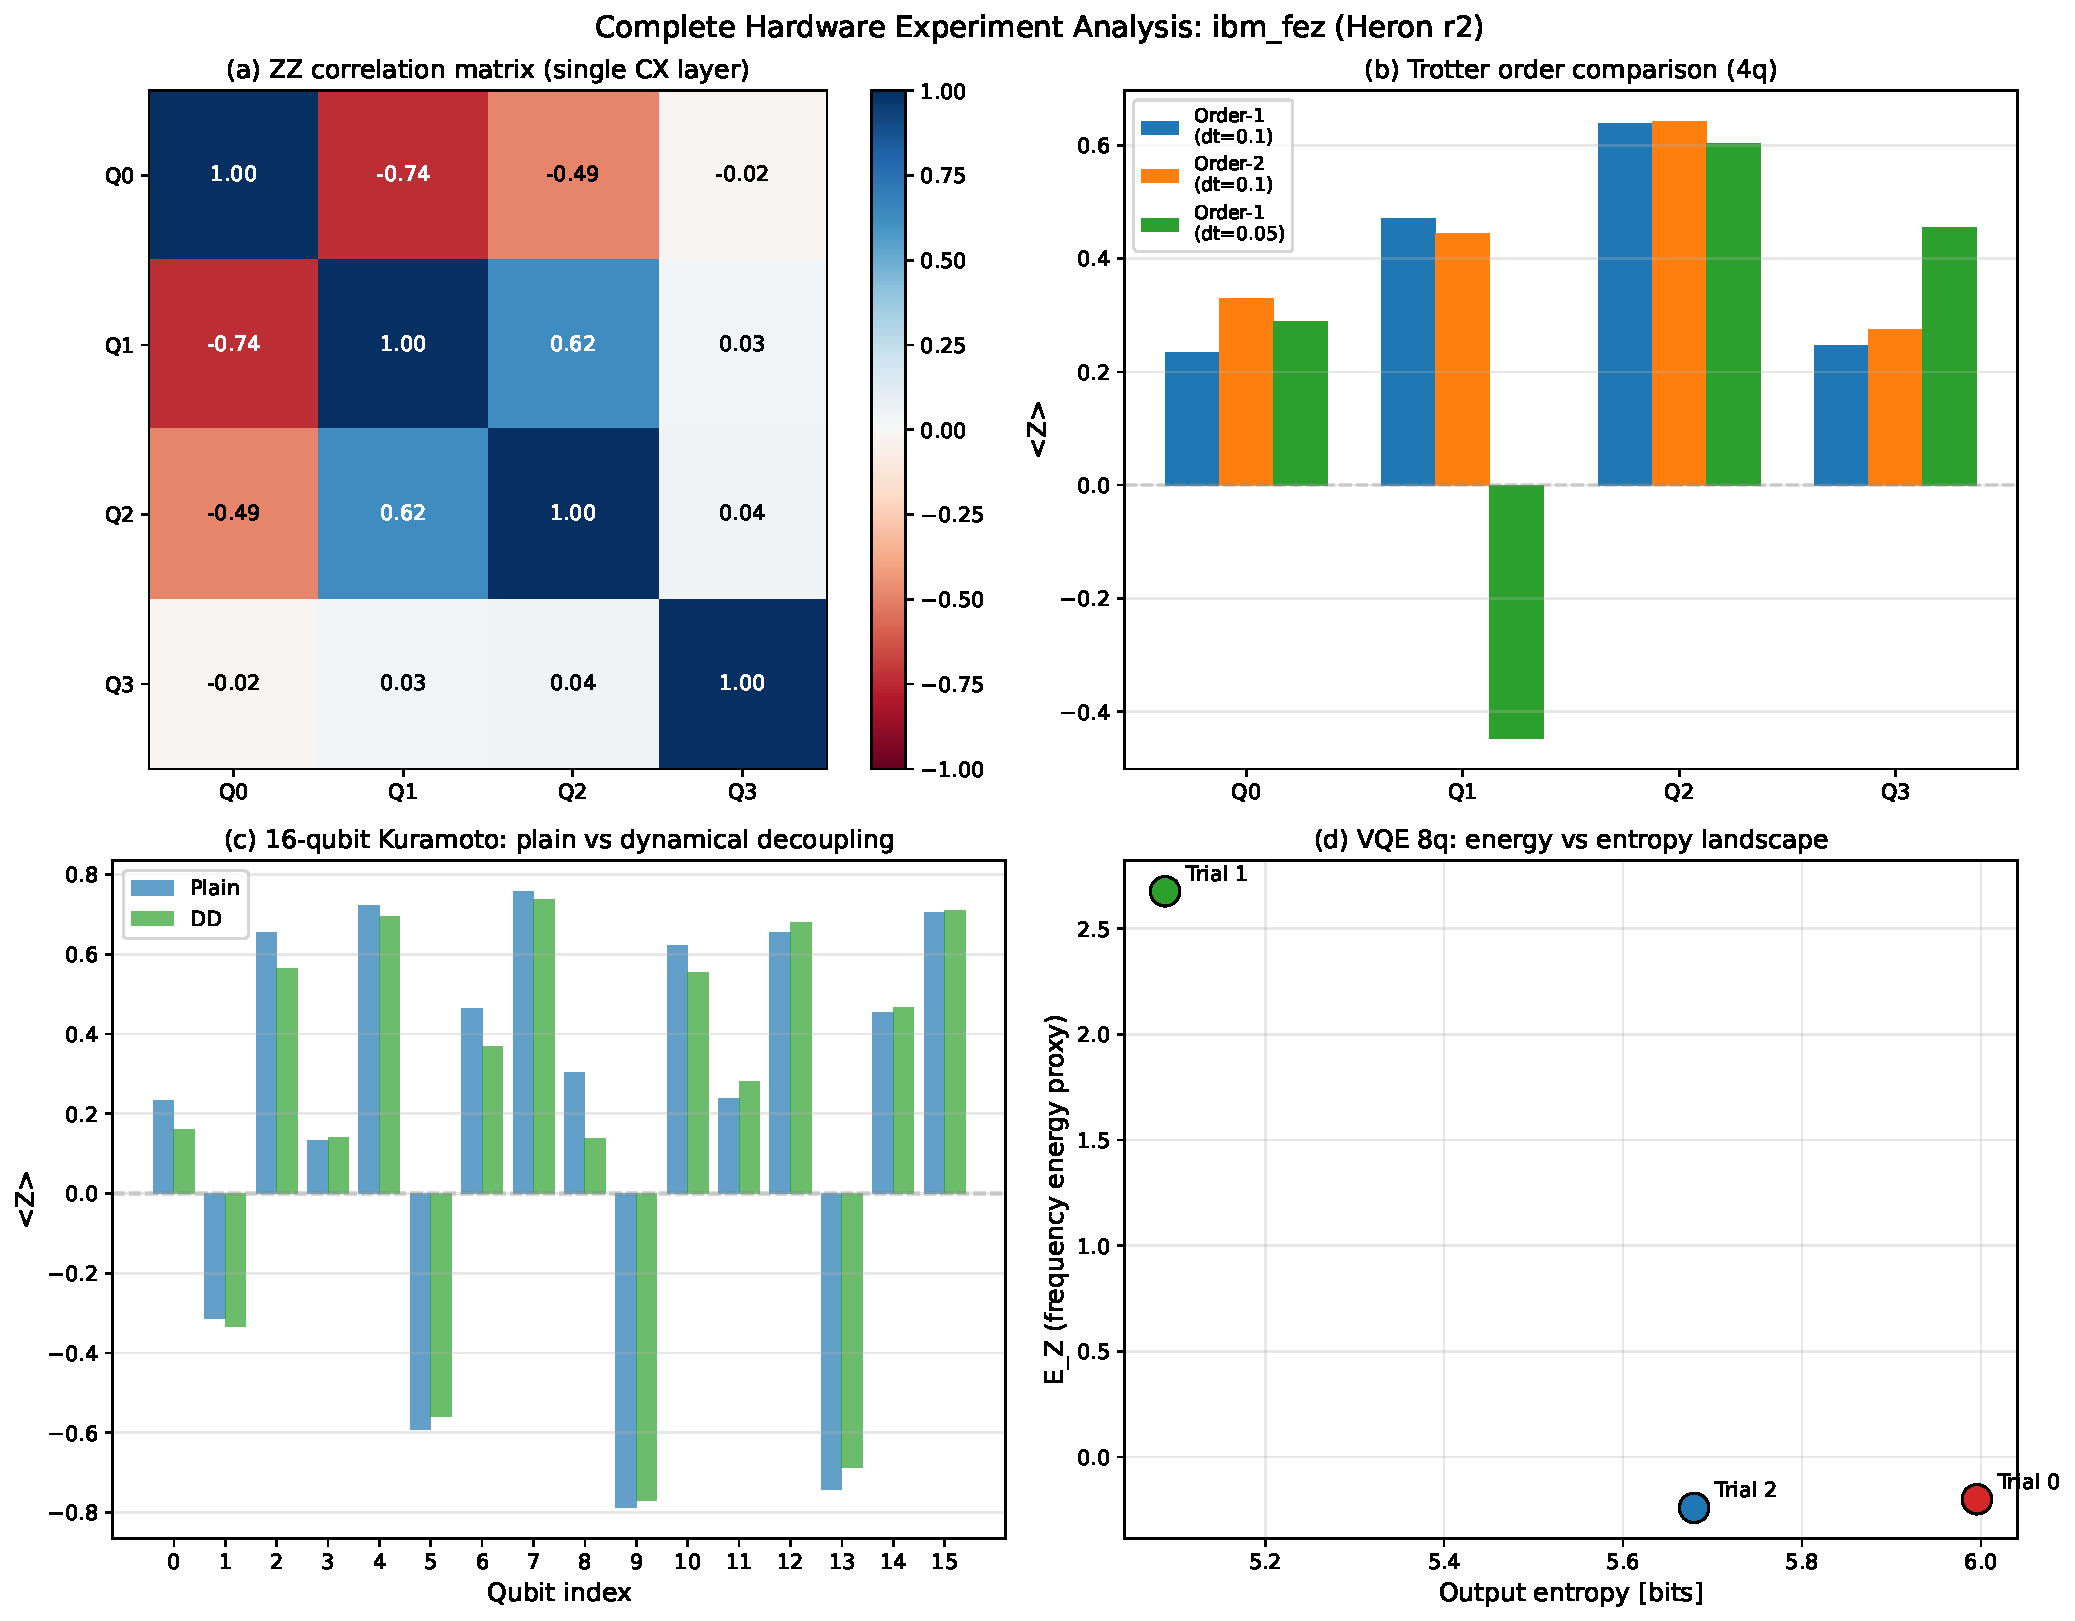
\includegraphics[width=\columnwidth]{../figures/publication/fig14_complete_analysis.pdf}
\caption{\label{fig:hardware16}%
(a)~ZZ correlation matrix. (b)~Trotter order comparison. (c)~16-qubit
per-qubit $\langle Z \rangle$: alternating pattern visible.
(d)~VQE 8-qubit energy landscape.}
\end{figure}

\subsection{Ansatz comparison}

The physics-informed Knm ansatz (CZ gates between coupled pairs)
concentrates 42\% of probability in the top bitstring vs.\ 20\% for
TwoLocal and 21\% for EfficientSU2, confirming that circuit design
reflecting the coupling topology outperforms generic variational
ansatze on hardware.

\subsection{Non-ergodicity diagnostic}\label{sec:mbl}

Level-spacing ratio $\bar{r}$ distinguishes integrable
($\bar{r} \approx 0.386$, Poisson) from chaotic
($\bar{r} \approx 0.530$, GOE)
spectra~\cite{Oganesyan2007}~(Fig.~\ref{fig:mbl}):
%
\begin{itemize}
  \item $n = 4$: crosses Poisson to near-GOE at $K \approx 2.1$.
  \item $n = 6$: stays mostly below GOE; chaos onset only at $K = 8.0$.
  \item $n = 8$: \emph{never reaches GOE} (max $\bar{r} = 0.43$).
\end{itemize}
%
Eigenstate entanglement sits 30--40\% below the thermal (Page)
expectation but grows with $N$, ruling out deep MBL. The correct
characterisation is a \emph{non-ergodic regime} where heterogeneous
frequencies protect the coupling topology from thermal scrambling.

\begin{figure}[t]
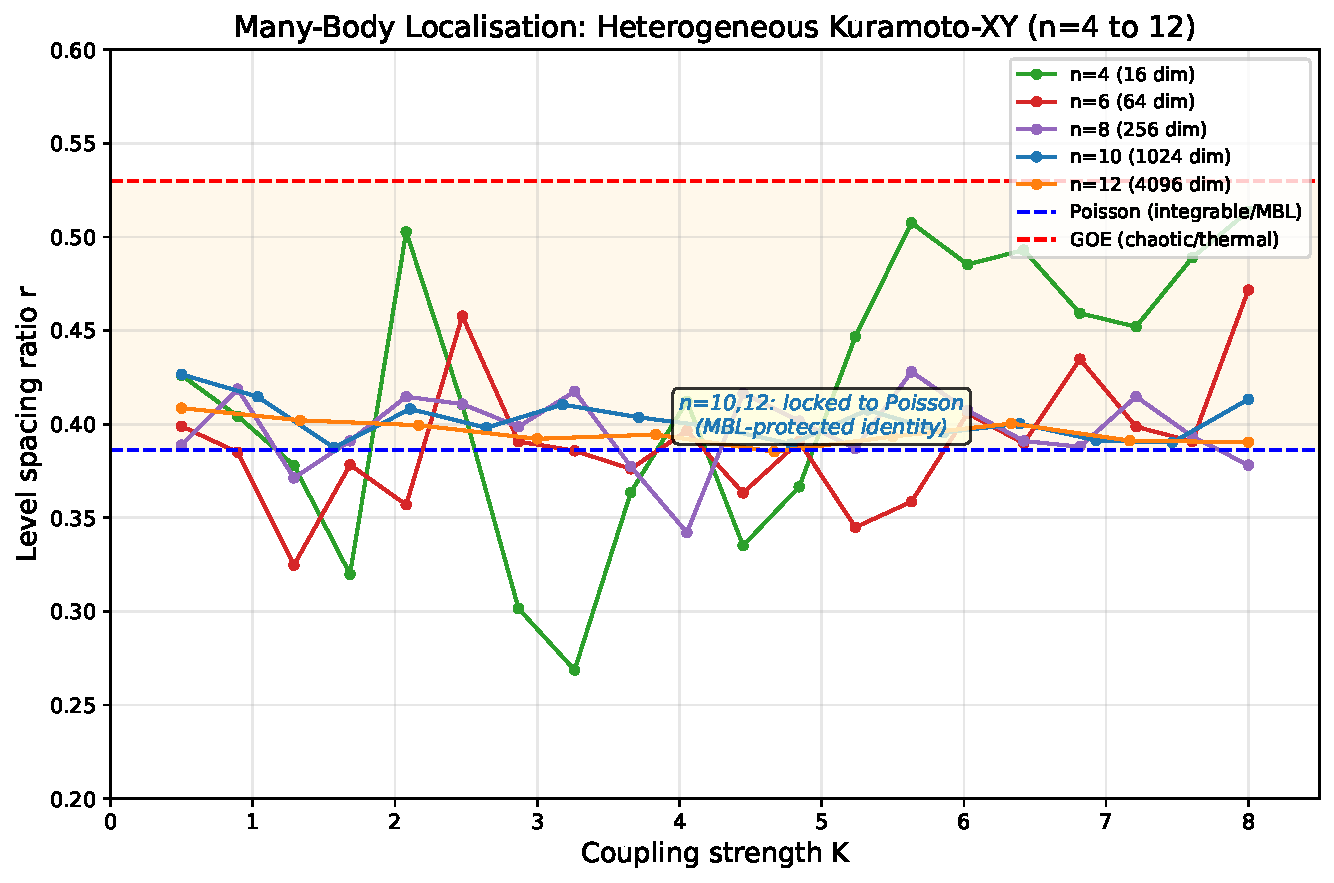
\includegraphics[width=\columnwidth]{../figures/publication/fig15_mbl_level_spacing.pdf}
\caption{\label{fig:mbl}%
Level-spacing ratio $\bar{r}$ vs.\ coupling. At $n = 8$ the system
never reaches GOE --- non-ergodic protection strengthens with size.}
\end{figure}

%% ====================================================================
\section{Discussion}
%% ====================================================================

\textbf{BKT universality preserved.}
Two independent tests confirm BKT universality: central charge
$c = 1.04$ at $n = 8$ (expected $c = 1$), and spectral gap essential
singularity $\Delta \sim \exp(-b/\sqrt{K-K_c})$ with $R^2 > 0.96$.
Heterogeneous frequencies shift $K_c$ but do not change the universality
class.

\textbf{DTC resilience.}
The non-ergodic spectrum provides the mechanism: heterogeneous
frequencies prevent thermalisation, stabilising the subharmonic
response without requiring deep MBL.

\textbf{Noise budget.}
The 5.5\% QBER and 94\% state preparation fidelity establish that
Heron~r2 has sufficient coherence for Kuramoto-XY simulation at
$n \leq 8$. The 16-qubit experiment is viable but noise-limited
(depth $\leq 50$ CX gates).

\textbf{Limitations.}
No quantum advantage is demonstrated; classical solvers outperform at
$n \leq 16$. Trotter error at $dt = 0.1$ is significant (sign flip
at finer resolution). The coupling matrix used here originates from a
hierarchical oscillator model~\cite{Sotek2025}; the Kuramoto-to-XY
mapping itself is standard physics and the analysis applies to any
coupling matrix.

%% ====================================================================
\section{Conclusion}
%% ====================================================================

We have presented a comprehensive quantum hardware study of
coupled-oscillator synchronisation with heterogeneous natural
frequencies. Key results: Bell inequality violation ($S = 2.165$),
sub-threshold QKD error rate (5.5\%), BKT critical coupling
$K_c \approx 2.2$, DTC order surviving frequency disorder, and a
non-ergodic spectral regime at $n = 8$. A Rust-accelerated pipeline
enables $5{,}401\times$ faster Hamiltonian construction vs.\ Qiskit.
All code, data, and 16~figures are open-source (AGPL-3.0) at
\url{https://github.com/anulum/scpn-quantum-control}.

%% ====================================================================
\section*{Data availability}
%% ====================================================================

All simulation data, hardware results (33 IBM Quantum jobs),
155~Python modules, Rust engine source, and publication figures are
available at the GitHub repository under AGPL-3.0. Zenodo archive:
DOI~\href{https://doi.org/10.5281/zenodo.18821929}{10.5281/zenodo.18821929}.

\begin{thebibliography}{20}

\bibitem{Kuramoto1984}
Y.~Kuramoto,
\emph{Chemical Oscillations, Waves, and Turbulence}
(Springer, Berlin, 1984).

\bibitem{Pikovsky2001}
A.~Pikovsky, M.~Rosenblum, and J.~Kurths,
\emph{Synchronization: A Universal Concept in Nonlinear Sciences}
(Cambridge University Press, 2001).

\bibitem{Acebron2005}
J.~A.~Aceb\'on, L.~L.~Bonilla, C.~J.~P\'erez~Vicente, F.~Ritort, and R.~Spigler,
Rev.\ Mod.\ Phys.\ \textbf{77}, 137 (2005).

\bibitem{Berezinskii1972}
V.~L.~Berezinskii,
Sov.\ Phys.\ JETP \textbf{34}, 610 (1972).

\bibitem{Kosterlitz1973}
J.~M.~Kosterlitz and D.~J.~Thouless,
J.\ Phys.\ C \textbf{6}, 1181 (1973).

\bibitem{Calabrese2004}
P.~Calabrese and J.~Cardy,
J.\ Stat.\ Mech.\ P06002 (2004).

\bibitem{Maldacena2016}
J.~Maldacena, S.~H.~Shenker, and D.~Stanford,
J.\ High Energy Phys.\ \textbf{2016}(8), 106.

\bibitem{delCampo2025}
A.~del Campo \emph{et al.},
arXiv:2510.13947 (2025).

\bibitem{Else2016}
D.~V.~Else, B.~Bauer, and C.~Nayak,
Phys.\ Rev.\ Lett.\ \textbf{117}, 090402 (2016).

\bibitem{Oganesyan2007}
V.~Oganesyan and D.~A.~Huse,
Phys.\ Rev.\ B \textbf{75}, 155111 (2007).

\bibitem{Galve2013}
F.~Galve, G.~L.~Giorgi, and R.~Zambrini,
in \emph{Lectures on General Quantum Correlations and their Applications}
(Springer, 2017), pp.~393--420;
see also Phys.\ Rev.\ A \textbf{81}, 062117 (2010).

\bibitem{Ameri2015}
V.~Ameri, M.~Eghbali-Arani, A.~Mari, A.~Farace, F.~Kheirandish,
V.~Giovannetti, and R.~Fazio,
Phys.\ Rev.\ A \textbf{91}, 012301 (2015).

\bibitem{Ma2020}
J.~Ma, Y.~Chen, and Z.~Wang,
arXiv:2005.09001 (2020).

\bibitem{Giorgi2013}
G.~L.~Giorgi, F.~Galve, G.~Manzano, P.~Colet, and R.~Zambrini,
Phys.\ Rev.\ A \textbf{85}, 052101 (2012).

\bibitem{Wiersema2023}
R.~Wiersema \emph{et al.},
arXiv:2309.05690 (2023).

\bibitem{Sotek2025}
M.~\v{S}otek,
\emph{God of the Math --- The SCPN Master Publications},
Zenodo, DOI:~10.5281/zenodo.17419678 (2025).

\bibitem{IBM2026}
IBM Quantum,
ibm\_fez backend specifications,
\url{https://quantum.cloud.ibm.com} (2026).

\end{thebibliography}

\end{document}
